\chapter{Úvod}
\label{sec:Introduction}

\begin{figure}[H]
\centering
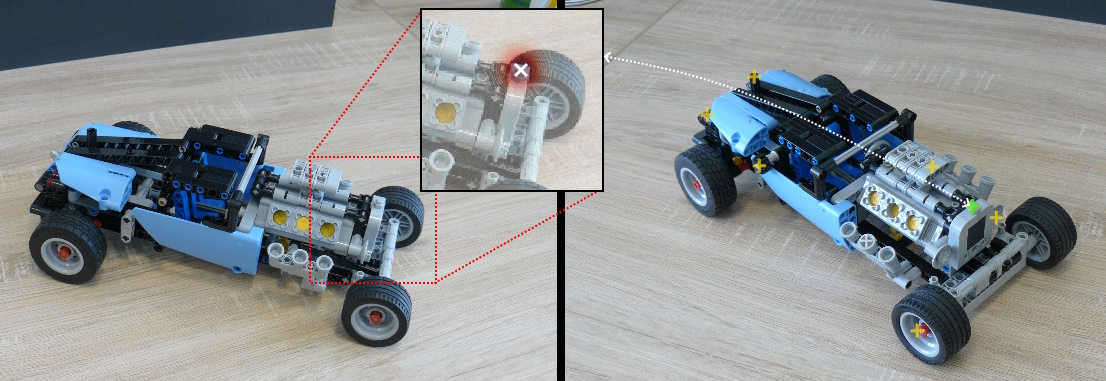
\includegraphics[width=1.0\textwidth,keepaspectratio]{Figures/bp_uvodni_obrazek.jpg}
\caption[Lokalizace klíčového bodu pro řešení PnP problému]{Lokalizace jednoho z klíčových bodů pro řešení PnP problému mezi reálným snímkem (vlevo) a syntetickým vykreslením (vpravo) se známými pozicemi klíčových bodů.}
\label{fig:bp_uvodni_obrazek}
\end{figure}


Lokalizace klíčových bodů zůstává nadále jedním z aktivně řešených problémů analýzy obrazu dnešní doby.
Klíčové body chápeme jako konkrétní body nacházející se na objektu zájmu, které chceme lokalizovat a následně sadu nalezených klíčových bodů použít pro další zpracování tykající se daného objektu zájmu, či jeho částí.

Využití lokalizace bodů nacházíme kupříkladu při odhadu postoje osob \cite{humanpose} nebo v biomedicínské technice \cite{unet}.
Při jejich následné lokalizaci musíme počítat s několika kvalitativně ovliňujícími členy v obrazu jako např. natočení kamery, vzdálenost, osvětlení, charakteristiky a kvalitu obrazu (zaostření) a ostatní vlivy prostředí okolo klíčového bodu. Kvůli tomuto musí techniky pro lokalizaci klíčových bodů být invariantní (tj. odolné vůči změnám ve vzhledu objektů), aby mohly spolehlivě fungovat i během změn vnějších podmínek mezi různými obrazy.

Cílem této bakalářské práce je \textbf{využít techniky lokalizace klíčových bodů pomocí hlubokých sítí U-Net} (a jejími následovníky či variacemi) pro zpřesnění 6 stupňů volnosti (DoF) transformace cílového objektu ve 3D prostoru pomocí PnP metod. PnP metody představují výpočetní techniky určené k řešení PnP problémů, které se zaměřují na přesný odhad polohy a orientace 3D objektů na základě korespondence lokalizovaných klíčových bodů na 2D snímku a známých pozicích klíčových bodů na 3D objektu.

Úloha lokalizace pro část vstupního snímku obsahující klíčový bod je ilustrována pomocí obrázku \ref{fig:bp_uvodni_obrazek}. Pro objekt byl detekován hrubý odhad pozice klíčového bodu. Klíčový bod je pomocí hluboké konvoluční neuronové sítě korektně lokalizován na lokaci s globálním maximem výsledku skalárního pole. Klíčový bod také byl korektně klasifikován s třídou známého klíčového bodu. Za předpokladu korektní lokalizace dostatečného počtu klíčových bodů můžeme orientaci objektu z levé části snímku odhadnout a vyjádřit pomocí 6 stupňů volnosti (DoF).

V rámci této práce byla prvně v \textbf{kapitole 2}  provedena \textbf{rešerše} existujících přístupů pro lokalizaci (a popř. korespondenci) klíčových bodů. Rešerše začíná od počátků analýzy obrazu pro obdobné úlohy (jako je např. SIFT) přes hluboké učení několika variací sítí U-Net až po state-of-art přístupy, jako je YOLOv8 či DINOv2. Detailně je popsán i modul STN, který slouží jako přídavný prvek do existujících sítí řešící prostorové transformace.

V \textbf{kapitole 3} je představen \textbf{dataset} určen pro trénink našich neuronových sítích. Jsou představeny dostupné snímky, informace a korespondující CSV soubory ke snímkům. Popány jsou také i některé detaily či poznatky týkající se datasetu. Následně v \textbf{kapitole 4} jsou popsány \textbf{zvolené přístupy} pro lokalizaci klíčových bodů, což je v případě této práce síť U-Net, U-Net++ a zakomponování modulu STN. Součástí jsou všechny detaily týkající se architektur implementovaných neuronových sítí, návrh ztrátové funkce, použití datasetu, augmentace dat a dalších relevantních částí týkající se návrhů. Přímě následuje \textbf{kapitola 5}, kde jsou popsány \textbf{detaily implementace} pomocí knihovny a trénovacího API TensorFlow 2. Popsán je příprava, průběh tréninků a také i zajímavé útržky implementace ztrátové funkce a modulu STN.

V \textbf{kapitole 6} jsou popsány \textbf{výsledky, evaluace, experimenty a dedukce} plynoucí z výsledků praktických úloh provedených v rámci této práce. Součástí je i samostatný experiment pomocí sítě DINOv2 od Meta AI. Finálně, v \textbf{kapitole 7} jsou popsány finální závěry a myšlenky plynoucí ze zjištění v této práci.
\endinput